\documentclass{book}

\usepackage[spanish]{babel}
\usepackage[utf8]{inputenc}
\usepackage[T1]{fontenc}
\usepackage{graphicx} 

\usepackage[
  top=3cm,
  bottom=3cm,
  left=2cm,
  right=2cm,
  heightrounded,
]{geometry}

\author{Ignacio Hernandez Valle}
\title{Biografia}
\date{\today}

\renewcommand{\labelitemi}{$\bullet$}

\begin{document}

\maketitle

\listoffigures
\addcontentsline{toc}{chapter}{Índice de figuras}


\chapter*{Jose Ignacio Hernandez Valle}


\chapter{Ignacio mi historia}
\section{Un poco sobre mi}

Me llamo Ignacio y soy estudiante de Ciencias de la Computacion naci en la Ciudad de Mexico tengo 20 años
Entre a esta carrera por medio de examen, para este llevo preparandome muchos meses ya que para entrar la cantidad de aciertos que piden es muy alta, estudie en la Prepa 6 pero tuve problemas en sexto año en la materia de quimica esto no me permitio concluir mi bachillerato ahí, para lograr tener mi certificado estuve inventigando las maneras que se ofrecen para concluir el bachillerato gracias a esto encontre el ``Examen Unico'' de Colegio de Bachilleres y logre terminar la preparatoria

\subsection{Hobbies}
\begin{enumerate}
  
\item Hacer ejercicio
\item Andar en moto y bicicleta
\item Escuchar musica
\end{enumerate}

\begin{figure}[h]
  \centering
  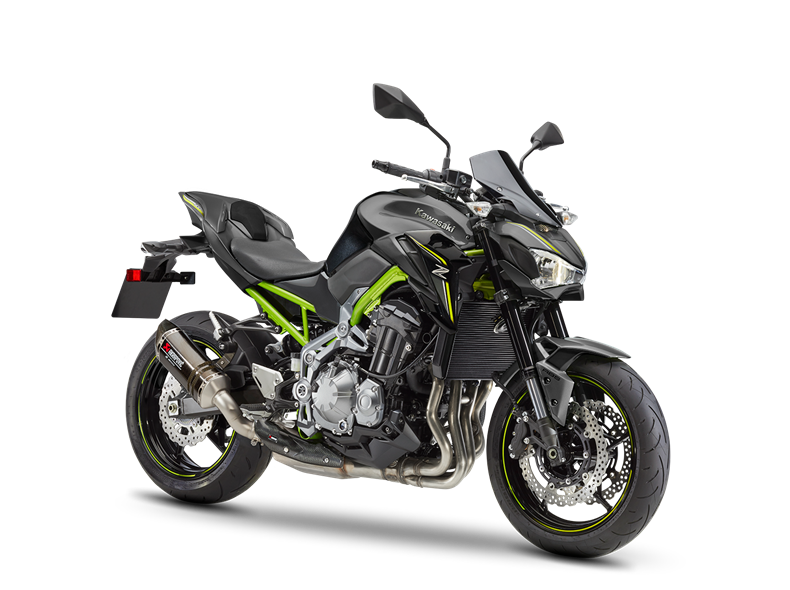
\includegraphics[scale=0.5]{IMG/8_1.png}
  \caption{\small Kawasaki z900 mi moto soñada} \label{fig:8_1}
\end{figure}

\begin{figure}[h]
  \centering
  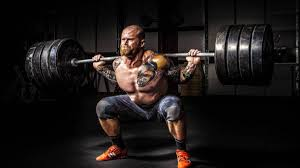
\includegraphics[scale=0.8]{IMG/8_2.jpg}
  \caption{\small Fitness } \label{fig:8_2}
\end{figure}



\end{document}
